\section{Mapping}
\label{sec:mapping}

Mapping relates atomistic and coarse-grained representations of the system. It is organized as follows: for each molecule {\em type} a mapping file is created. When used as a command option, these files are combined in a list separated by a semicolon, e.~g. \progopt{--cg}~\texttt{"protein.xml;solvent.xml"}.

Each mapping file contains a {\em topology} of the coarse-grained molecule and a list of {\em maps}. Topology specifies coarse-grained beads and bonded interactions between them. Each coarse-grained bead has a name, type, a list of atoms which belong it, and a link to a map. A map is a \hyperref[sec:mapping_operator]{set of weights} $c_{Ii}$ for an atom $i$ belonging to the bead $I$. It is used to calculate the position of a coarse-grained bead from the positions of atoms which belong to it. Note that $c_{Ii}$ will be automatically re-normalized if their sum is not equal to 1, i.~e. in the case of a center-of-mass mapping one can simply specify atomic masses. 
A complete reference for mapping file definitions can be found in sec.~\ref{sec:ref_mapping}.

As an example, we will describe here a mapping file of a united atom model of a propane molecule. In this coarse-grained model two bead types (A,B) and three beads (A1, B1, A2) are defined, as shown in fig.~\ref{fig:propane_map}. We will use centers of mass of the beads as  coarse-grained coordinates.


\begin{figure}[ht]
  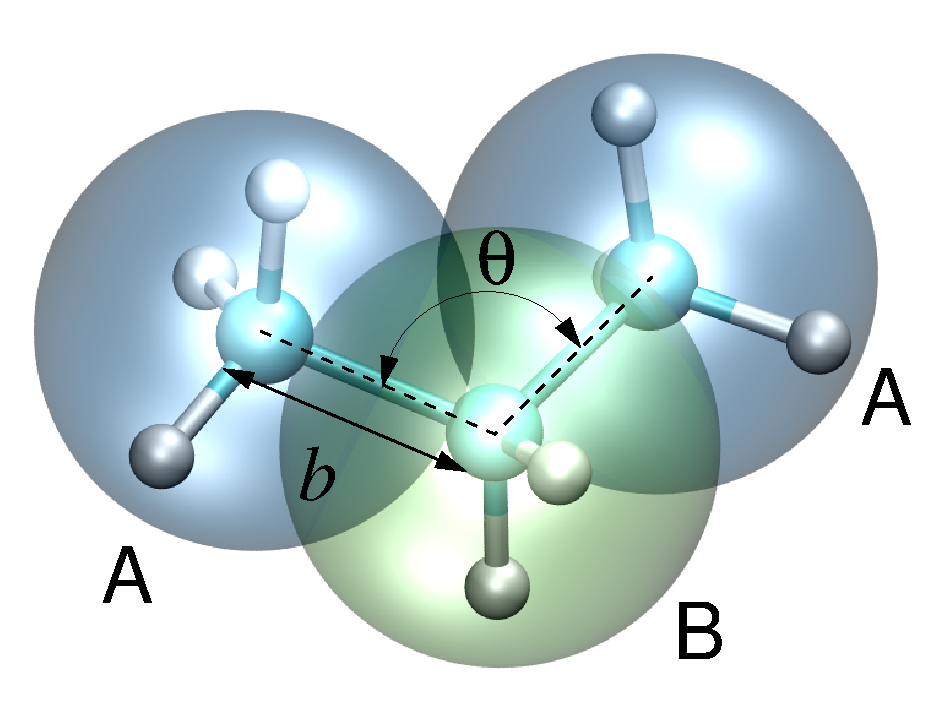
\includegraphics[width=0.4\textwidth]{functionality/fig/propane.eps}
  \caption{Mapping for propane
  \label{fig:propane_map}
}
\end{figure}

\lstinputlisting{functionality/propane.xml}

The \mapopt{ident} tag in the mapping definition must match the name of the molecule in the reference system.

The name must be unique within the mapping file. Type defines the type of the bead. The \hyperlink{\mapref{topology.cg_beads.cg_bead.mapping}}{mapping} tag defines which mapping scheme is used from the mapping section in the file.

Type and mapping can be different since the number of atoms for the same bead type may differ, e.g. at chain ends for saturating hydrogen atoms.

In the \hyperlink{\mapref{topology.cg_beads.cg_bead.mapping}}{mapping section}, the mapping operator is defined. Currently this includes only weights for a linear mapping scheme.

To map from an atomistic to a reference system, \prog{csg_map} can be used:
\begin{verbatim}
  csg_map --top topol.tpr --trj traj.trr --cg "protein.xml;solvent.xml" --out cg.gro
\end{verbatim}

To create a coarse-grained topology based on the mapping scheme, see \prog{csg_gmxtopol}.
